%!TeX root=MemoriaTFG.tex

\section{Bloc 2: representació de l'estat i memòria}
\label{sec:bloc2}

Amb els dos agents \ac{SB3} seleccionats al Checkpoint~1, el segon bloc explora dues
direccions ortogonals per superar el sostre de rendiment: millorar la \emph{representació}
de l'estat (Fase~3, dividida en arquitectura i inicialització del cos) i dotar l'agent de
\emph{memòria} entre mans (Fase~4). El Checkpoint~2 tanca el bloc fixant el model que
s'adopta per a desplegament.

\subsection{Fase 3: el feature extractor COS}
\label{sec:fase3}

\begin{sloppypar}
La Fase~3 estudia \texttt{CosMultiInput}, un \emph{feature extractor} convolucional
propi, com a alternativa a l'extractor pla per defecte de \ac{SB3}.
L'estudi respon dues preguntes acoblades: si l'\textbf{arquitectura} convolucional
aporta valor per si sola (Q1, secció~\ref{sec:fase3-arq}) i si
\textbf{inicialitzar-la} amb coneixement previ del joc desbloqueja un rendiment
superior (Q2, secció~\ref{sec:fase3-init}).
\end{sloppypar}

\subsubsection{Arquitectura: CNN vs MLP}
\label{sec:fase3-arq}

\paragraph{Hipòtesi.} El vector pla de 240~dimensions amaga l'estructura espacial del
tensor de cartes. Un \ac{MLP} pla ha de \emph{redescobrir} per ell mateix que el 4~de
Copes i el 4~d'Ors comparteixen rang, o que cartes de pals diferents poden tenir forces
relacionades. La hipòtesi (Q1) és que un extractor que respecta l'estructura
\(6 \times 4 \times 9\) del tensor de cartes (mitjançant convolucions) supera el \ac{MLP}
estàndard.

\paragraph{Disseny.}

\emph{L'extractor CosMultiInput.} Per provar la hipòtesi es
dissenya \texttt{CosMultiInput} (\texttt{RL/models/core/feature\_extractor.py}), un
extractor de dues branques (figura~\ref{fig:cos-multi-input}). La branca \acf{CNN} aplica
dues convolucions sobre el tensor \((6,4,9)\) (taula~\ref{tab:canals-cartes}): la primera amb nucli \(1\times3\) detecta
patrons entre rangs consecutius; la segona amb nucli \(3\times3\) integra la informació
entre pals i rangs, produint 320~dimensions. La branca densa projecta el vector de context
de 24~dimensions (taula~\ref{tab:context-obs}) a~32. Les dues sortides es concatenen i es projecten a 256~dimensions. La
sortida coincideix amb l'amplada de la primera capa oculta de la política
(\texttt{net\_arch=[256,256]}), de manera que \texttt{CosMultiInput} substitueix
l'extractor per defecte de \ac{SB3} (\texttt{CombinedExtractor}, que simplement aplana
l'observació) sense cap altre canvi. L'adaptador \texttt{CosMultiInputSB3} (\texttt{RL/%
\allowbreak{}models/\allowbreak{}sb3/\allowbreak{}sb3\_\allowbreak{}features\_%
\allowbreak{}extractor.py}) fa de pont entre el vector pla i les dues branques.

\begin{figure}[H]
  \centering
  \resizebox{\textwidth}{!}{%
  \begin{tikzpicture}[
      inp/.style ={draw, rounded corners=3pt, minimum width=2.2cm, minimum height=0.85cm,
                   align=center, font=\small, fill=blue!6},
      cnn/.style ={draw, rounded corners=3pt, minimum width=2.5cm, minimum height=0.75cm,
                   align=center, font=\footnotesize, fill=orange!10},
      ctx/.style ={draw, rounded corners=3pt, minimum width=2.5cm, minimum height=0.75cm,
                   align=center, font=\footnotesize, fill=teal!10},
      fus/.style ={draw, rounded corners=3pt, minimum width=2.5cm, minimum height=0.75cm,
                   align=center, font=\footnotesize, fill=purple!8},
      res/.style ={draw, rounded corners=3pt, minimum width=2.2cm, minimum height=0.85cm,
                   align=center, font=\small, fill=blue!6},
      arr/.style ={-{Stealth}, thick},
  ]
    % ── Branca CNN (fila superior) ─────────────────────────────────────────
    \node[inp] (cartes) {Tensor cartes\\$(6,4,9)$};
    \node[cnn, right=0.8cm of cartes]  (cnn1) {\texttt{Conv2d}\\$6{\to}16$, $1{\times}3$};
    \node[cnn, right=0.7cm of cnn1]   (cnn2) {\texttt{Conv2d}\\$16{\to}32$, $3{\times}3$};
    \node[cnn, right=0.7cm of cnn2]   (flat) {Flatten\\${\to}\,320$};

    % ── Branca context (fila inferior) ────────────────────────────────────
    \node[inp, below=1.6cm of cartes] (context) {Vector context\\$(24,)$};
    \node[ctx, right=0.8cm of context] (lin) {\texttt{Linear}\\$24{\to}32$};

    % ── Fusió ──────────────────────────────────────────────────────────────
    \node[fus, right=1.2cm of flat |- context, yshift=0.8cm]
          (cat)   {cat$([320,\,32])$\\$=352$};
    \node[fus, right=0.7cm of cat]  (fusio) {\texttt{Linear}\\$352{\to}256$};
    \node[res, right=0.7cm of fusio] (latent) {Latent\\$(256,)$};

    % ── Fletxes CNN ────────────────────────────────────────────────────────
    \draw[arr] (cartes)  -- (cnn1);
    \draw[arr] (cnn1)    -- (cnn2);
    \draw[arr] (cnn2)    -- (flat);
    \draw[arr] (flat)    -- (cat);

    % ── Fletxes context ────────────────────────────────────────────────────
    \draw[arr] (context) -- (lin);
    \draw[arr] (lin)     -| (cat);

    % ── Fletxes fusió ──────────────────────────────────────────────────────
    \draw[arr] (cat)   -- (fusio);
    \draw[arr] (fusio) -- (latent);
  \end{tikzpicture}%
  }
  \caption{\texttt{CosMultiInput}: arquitectura de dues branques. La branca CNN processa
           el tensor de cartes $(6,4,9)$; la branca lineal el vector de context $(24,)$.
           Les sortides es concatenen i es projecten a un vector latent de 256~dimensions.}
  \label{fig:cos-multi-input}
\end{figure}

\emph{Els tres protocols.} La comparació es fa sobre els tres protocols d'entrenament
introduïts a la Fase~2 (secció~\ref{sec:fase2}), que es recorden aquí perquè ara es
comparen tots tres:
\begin{itemize}
  \item \textbf{Control}: entrenar directament sobre \emph{partides senceres}; la condició
        de referència, sense cap facilitació.
  \item \textbf{Curriculum}: entrenar primer sobre \emph{mans} i després fer \emph{finetune}
        sobre partides senceres (el currículum de dues etapes de la Fase~2).
  \item \textbf{Mans}: entrenar \emph{exclusivament} sobre mans individuals, sense el pas
        posterior a partides.
\end{itemize}

\emph{Comparació experimental.} Per a cada protocol i agent es compara la variant COS (amb
pesos aleatoris) amb la variant \ac{MLP}, amb 24~milions de passos cada combinació i la
mateixa distribució d'oponents que la Fase~2 (10\% Random + 90\% Regles). Això suposa sis
runs nous amb COS i dos amb \ac{MLP} sobre mans; les quatre sèries \ac{MLP} de control i
curriculum es reutilitzen de la Fase~2 per no reentrenar-les.

\paragraph{Resultats.} El COS amb pesos aleatoris no supera sistemàticament el \ac{MLP}
(taula~\ref{tab:fase3}). Només aporta una millora clara al protocol de control per a
DQN-SB3 (+10{,}5~punts). El protocol \textbf{mans} torna a ser el millor en termes
absoluts (totes les combinacions superen el 82\%), però la diferència entre COS i \ac{MLP}
hi és marginal (\(<4\) punts). La inducció estructural per si sola, amb pesos aleatoris,
no és suficient per desbloquejar un avantatge. La lectura és coherent: al protocol de
control, sense cap facilitació, la capacitat addicional de la \ac{CNN} per extreure
patrons de l'estructura de les cartes es tradueix en un guany real; al protocol de mans,
el currículum d'entrenament sobre mans individuals ja exposa l'agent als patrons
carta-a-carta en un context simplificat, de manera que el \ac{MLP} arriba al protocol
de mans amb una representació prou rica i la \ac{CNN} no hi aporta res addicional.

\begin{table}[H]
  \centering
  \begin{tabular}{llrrr}
    \toprule
    Protocol & Agent & COS & \ac{MLP} & $\Delta$ \\
    \midrule
    Control    & DQN-SB3 & 71{,}0\% & 60{,}5\% & $+10{,}5$ \\
    Control    & PPO-SB3 & 32{,}5\% & 35{,}0\% & $-2{,}5$ \\
    Curriculum & DQN-SB3 & 56{,}2\% & 56{,}0\% & $+0{,}2$ \\
    Curriculum & PPO-SB3 & 63{,}0\% & 75{,}0\% & $-12{,}0$ \\
    Mans       & DQN-SB3 & 82{,}2\% & 85{,}8\% & $-3{,}6$ \\
    Mans       & PPO-SB3 & 89{,}0\% & 87{,}2\% & $+1{,}8$ \\
    \bottomrule
  \end{tabular}
  \caption{Pic de \texttt{metric} (24M passos) per a COS amb pesos aleatoris vs \ac{MLP}.}
  \label{tab:fase3}
\end{table}

\begin{figure}[H]
  \centering
  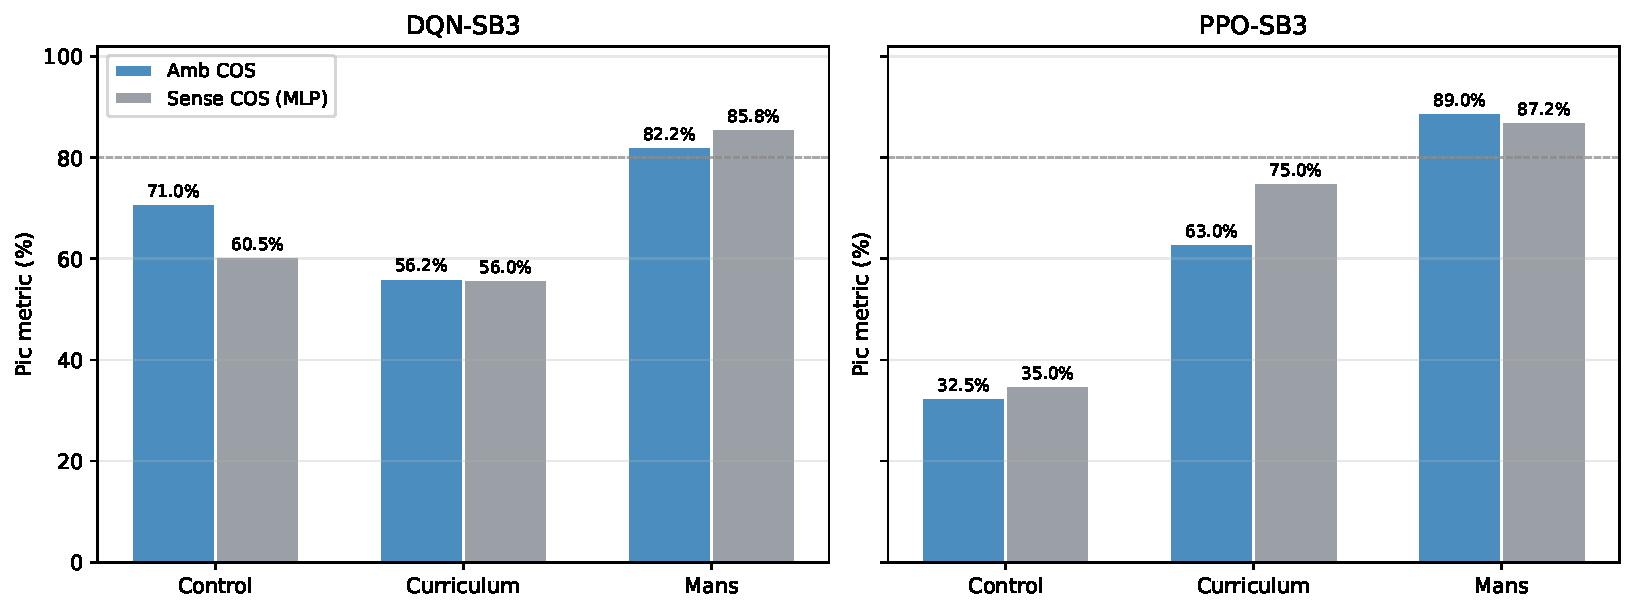
\includegraphics[width=\textwidth]{figures/fase3/fase3_cos_vs_mlp.pdf}
  \caption{Pic de \texttt{metric} (24M passos) per protocol i agent, COS amb pesos
           aleatoris vs \ac{MLP}. La línia discontínua marca el 80\%. El COS només supera
           clarament el \ac{MLP} al control de DQN-SB3; al protocol de mans (el millor en
           absolut) la diferència és marginal.}
  \label{fig:fase3-cos-mlp}
\end{figure}

\paragraph{Decisió.} Es fixa el protocol de mans per a la resta del bloc. Com que el COS
amb pesos aleatoris no arrenca amb cap avantatge representacional, la pregunta natural és
si \emph{inicialitzar-lo} amb coneixement previ del joc canvia el resultat. Això motiva la
subsubsecció següent.

\subsubsection{Inicialització supervisada del cos}
\label{sec:fase3-init}

\paragraph{Hipòtesi.} Un cos preentrenat que ja distingeix rang, pal i força de les
cartes des del primer pas d'\ac{AR} permet a la política concentrar-se en la presa de
decisions en lloc de reaprendre la representació. La pregunta (Q2) és doble: aporta valor el
preentrenament supervisat, i quin règim (congelat o ajustat) és preferible?

\paragraph{Disseny.}

\emph{El preentrenament supervisat.} La idea és donar al cos \texttt{CosMultiInput}
una representació útil de les cartes \emph{abans} que comenci l'\ac{AR}, per tal que
l'agent no hagi de descobrir l'estructura del joc i la política al mateix temps. Per
aconseguir-ho, s'afegeix temporalment al cos el model \texttt{ModelPreEntrenament}, que
hi acobla tres caps de predicció (taula~\ref{tab:caps-preentrenament}): la força de cada
carta de la mà, la màscara d'accions legals i la puntuació d'envit
(figura~\ref{fig:sl-preentrenament}).

\begin{figure}[H]
  \centering
  \begin{tikzpicture}[
    bloc/.style ={draw, rounded corners=3pt, minimum width=2.0cm,
                  minimum height=0.75cm, align=center, font=\small},
    headbox/.style={draw, rounded corners=3pt, minimum width=2.6cm,
                  minimum height=0.65cm, align=center, font=\footnotesize,
                  fill=green!8},
    >=Stealth, thick
  ]
    \node[bloc, fill=gray!10]   (ds)  {Dataset\\200k estats};
    \node[bloc, right=1.4cm of ds,  fill=orange!10] (cos) {COS\\(backbone)};
    \node[bloc, right=1.2cm of cos, fill=purple!8]  (lat) {Latent\\$(256)$};

    \node[headbox, above right=0.55cm and 1.1cm of lat] (cf) {\texttt{cap\_forces}\\MSE};
    \node[headbox, right=1.1cm of lat]                  (ca) {\texttt{cap\_accions}\\BCE};
    \node[headbox, below right=0.55cm and 1.1cm of lat] (ce) {\texttt{cap\_envido}\\MSE};
    \draw[->] (ds)  -- (cos);
    \draw[->] (cos) -- (lat);
    \draw[->] (lat.north east) -- (cf.west);
    \draw[->] (lat.east)       -- (ca.west);
    \draw[->] (lat.south east) -- (ce.west);

    \draw[->, dashed, gray!60] (lat.west) --
          node[above, font=\scriptsize]{$\nabla\mathcal{L}$} (cos.east);
  \end{tikzpicture}
  \caption{Esquema del preentrenament supervisat: els tres caps propaguen gradient al cos
           i l'obliguen a aprendre representacions sensibles a l'estructura del joc.
           Un cop acabat, els caps es descarten i es conserven només els pesos del cos.}
  \label{fig:sl-preentrenament}
\end{figure}

El dataset es genera jugant partides amb una política pseudo-aleatòria sobre l'entorn
real: a cada pas es registra l'observació de l'agent i s'extreuen automàticament les
etiquetes del propi motor de joc (la força de cada carta via \texttt{TrucJudger}, la
màscara d'accions legals de l'estat actual i els punts d'envit de la mà inicial). El
resultat són 200\,000~transicions amb un repartiment 80/20 entre entrenament i validació;
la pèrdua combinada pondera els tres objectius
(\(1{,}0\cdot\mathcal{L}_{\text{envit}} + 2{,}0\cdot\mathcal{L}_{\text{accions}} +
2{,}5\cdot\mathcal{L}_{\text{forces}}\)), donant més pes als objectius que exigeixen una
comprensió més fina de l'estructura de les cartes. Un cop acabat l'entrenament supervisat,
els caps es descarten; la seva única funció era proporcionar gradient informatiu al cos,
i el que es conserva és el coneixement que el cos ha consolidat als seus pesos.

\begin{table}[H]
  \centering
  \begin{tabular}{llcl}
    \toprule
    Cap & Sortida & Mida & Pèrdua \\
    \midrule
    \texttt{cap\_envido}          & Punts d'envit de la mà      & 1  & MSE \\
    \texttt{cap\_accions\_legals} & Màscara d'accions legals    & 19 & BCE \\
    \texttt{cap\_forces}          & Força de cada carta a la mà & 3  & MSE \\
    \bottomrule
  \end{tabular}
  \caption{Caps de predicció del \texttt{ModelPreEntrenament} per al preentrenament
           supervisat del cos \texttt{CosMultiInput}.}
  \label{tab:caps-preentrenament}
\end{table}

\emph{Els quatre règims.} El coneixement preentrenat es pot aprofitar de maneres
diferents, que constitueixen la variable d'estudi de la fase:
\begin{itemize}
  \item \textbf{Sense COS (MLP)}: l'extractor pla per defecte de \ac{SB3}, sense cap
        inducció estructural; estableix el sostre d'un model sense coneixement de
        l'estructura de les cartes.
  \item \textbf{Scratch} (des de zero): el COS amb \emph{pesos aleatoris}; la \ac{CNN} ha
        d'aprendre la representació de les cartes alhora que la política.
  \item \textbf{Frozen} (congelat): el COS amb \emph{pesos preentrenats supervisadament i
        congelats}; la representació és fixa i estable, i només s'entrena la política.
  \item \textbf{Finetune} (ajust fi): el COS amb pesos preentrenats que \emph{es continuen
        ajustant} durant l'\ac{AR}; té millor potencial però arrisca a oblidar la
        representació inicial.
\end{itemize}
Cada comparació aïlla un efecte: \emph{scratch} contra \ac{MLP} mesura l'efecte de
l'arquitectura, i \emph{frozen}/\emph{finetune} contra \emph{scratch} mesuren l'efecte del
preentrenament.

\paragraph{Resultats.} El règim \textbf{frozen és el millor}
(taula~\ref{tab:fase35}). Per a DQN-SB3 assoleix el 91{,}2\% (+5{,}4~punts sobre el
\ac{MLP}, +9 sobre \emph{scratch}): el cos preentrenat i congelat actua com a extractor
estable que permet a la xarxa de valor aprendre sense interferències. El \emph{finetune}
degrada respecte al \emph{frozen} en tots dos agents: el gradient de l'\ac{AR} deteriora
parcialment la representació preentrenada. Per a PPO-SB3 els quatre règims convergeixen
entre 87--89\%, de manera que el preentrenament hi aporta poc.

\begin{table}[H]
  \centering
  \begin{tabular}{lrr}
    \toprule
    Règim & DQN-SB3 & PPO-SB3 \\
    \midrule
    Sense COS (\ac{MLP}) & 85{,}8\% & 87{,}2\% \\
    Scratch              & 82{,}2\% & 89{,}0\% \\
    Frozen               & \textbf{91{,}2\%} & \textbf{89{,}5\%} \\
    Finetune             & 88{,}5\% & 88{,}0\% \\
    \bottomrule
  \end{tabular}
  \caption{Pic de \texttt{metric} (protocol mans, 24M passos) per als quatre règims
           d'inicialització del cos.}
  \label{tab:fase35}
\end{table}

\paragraph{Decisió.} El preentrenament supervisat aporta valor real, però només quan el
cos queda \textbf{congelat}. S'adopta el COS preentrenat i congelat com a \emph{backbone}
estable per a la fase següent.

\subsection{Fase 4: memòria d'oponent (LSTM) i pool d'oponents}
\label{sec:fase4}

\paragraph{Hipòtesi (Q3).} Totes les fases anteriors entrenen contra un oponent fix i amb
un agent sense estat intern. La Fase~4 introdueix dues variables: una memòria seqüencial \acf{LSTM}
que manté estat entre mans, i un \emph{pool} de sis variants d'oponent
(taula~\ref{tab:pool-variants}). Se'n deriven tres hipòtesis concretes:
\begin{itemize}
  \item \textbf{H1}: L'\ac{LSTM} millora el rendiment global respecte a un agent sense
        memòria entrenat amb les mateixes condicions.
  \item \textbf{H2}: L'agent amb \ac{LSTM} mostra adaptació progressiva dins la sessió:
        el win-rate creix de la mà~1 a la mà~5 a mesura que l'agent infereix el patró de
        l'oponent.
  \item \textbf{H3}: El pool de sis variants no perjudica significativament la convergència
        d'un agent sense memòria (F4-ablació comparable a les línies base de la Fase~3.5).
\end{itemize}

\paragraph{Disseny.}

\emph{El pool d'oponents.} En lloc d'un oponent fix, l'agent s'entrena contra sis variants
d'\texttt{AgentRegles} amb estils contrastats (taula~\ref{tab:pool-variants}). La diversitat
és deliberada: amb un únic oponent existiria una política mitjana òptima que un agent sense
memòria podria memoritzar; amb sis estils clarament diferents no n'hi ha cap, de manera que
l'única manera de jugar bé contra tots és \emph{detectar} qui es té al davant i adaptar-s'hi.

\emph{Sessions multi-mà.} Per donar marge a aquesta adaptació, l'episodi d'\ac{AR} deixa de
ser una mà i passa a ser una \emph{sessió} de \(N=5\) mans consecutives contra el mateix
oponent. El nou entorn \texttt{TrucGymEnvSessio} envolta \texttt{TrucGymEnvMa} i
\emph{intercepta} els senyals de final (\texttt{terminated}) intermedis, de manera que
l'estat de l'\ac{LSTM} no es reinicia fins al final de les cinc mans; al començament de cada
sessió es mostreja un oponent nou del pool.

\emph{L'arquitectura amb memòria.} La cadena de processament és
obs(240)~$\rightarrow$~COS congelat(256)~$\rightarrow$~\ac{LSTM}(256)~$\rightarrow$~\ac{MLP}
lleuger~$\rightarrow$~caps de política i valor. S'usa \texttt{RecurrentPPO} (de
\texttt{sb3\_contrib}) amb \emph{retropropagació en el temps truncada}
(secció~\ref{sec:recurrencia}) sobre seqüències, on el \texttt{batch\_size} es mesura en seqüències
i no en transicions individuals. No s'usa \acs{DRQN} (l'anàleg basat en la funció de valor)
perquè requeriria un \emph{replay buffer} seqüencial no disponible a \ac{SB3}.

\emph{Pressupost i avaluació.} Es comparen dos runs nous amb les línies base de la Fase~3.5:
\textbf{F4-ablació} (PPO + COS congelat + pool, sense memòria) i \textbf{F4-complet}
(\texttt{RecurrentPPO} amb \ac{LSTM} sobre el COS congelat + pool); la primera comparació
aïlla l'efecte del pool i la segona, l'efecte de la memòria. Cada run nou s'entrena 12M
passos, la meitat que a la Fase~3.5, perquè la retropropagació en el temps encareix molt el
còmput. L'avaluació, a més de la \texttt{metric} habitual, acumula el win-rate \emph{per
posició dins la sessió} (de la mà~1 a la~5) per detectar si l'agent millora a mesura que
coneix l'oponent.

\paragraph{Resultats.} Cap de les tres hipòtesis es valida plenament
(taula~\ref{tab:fase4}). Les figures~\ref{fig:fase4-corbes} i~\ref{fig:fase4-barplot}
mostren l'evolució i els pics de \texttt{metric}; la figura~\ref{fig:fase4-adaptacio}
detalla el win-rate per posició dins la sessió, clau per a H2.

\begin{figure}[H]
  \centering
  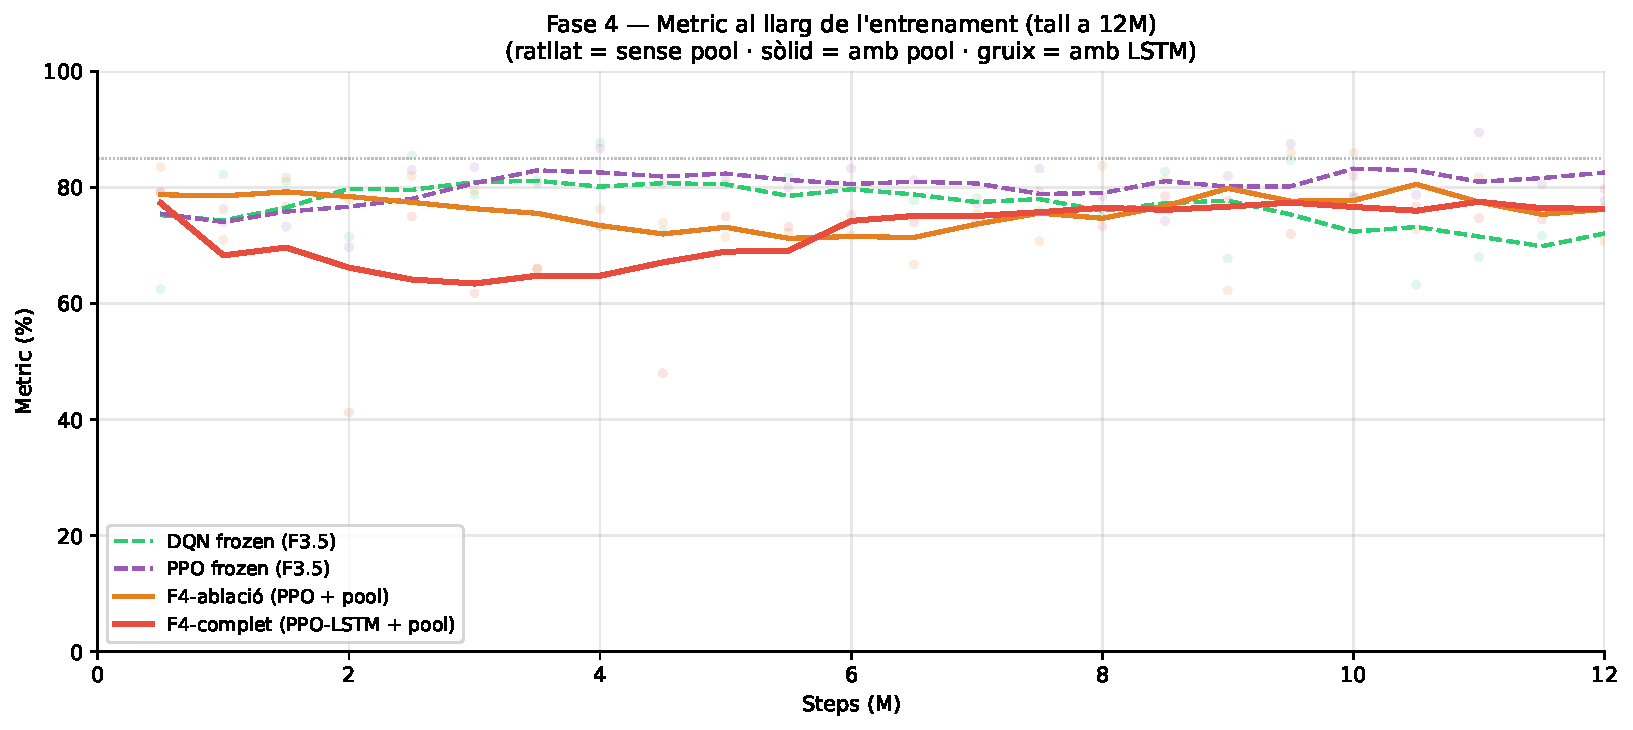
\includegraphics[width=0.82\textwidth]{figures/fase4/fase4_corbes.pdf}
  \caption{Evolució de la \texttt{metric} al llarg de l'entrenament per als quatre runs de
           la Fase~4, tallats a 12M passos. Línies discontínues: línies base de la Fase~3.5
           (sense pool); línies sòlides: runs amb pool; gruix addicional: model amb
           \ac{LSTM}. La línia puntejada gris marca el 85\%.}
  \label{fig:fase4-corbes}
\end{figure}

\begin{figure}[H]
  \centering
  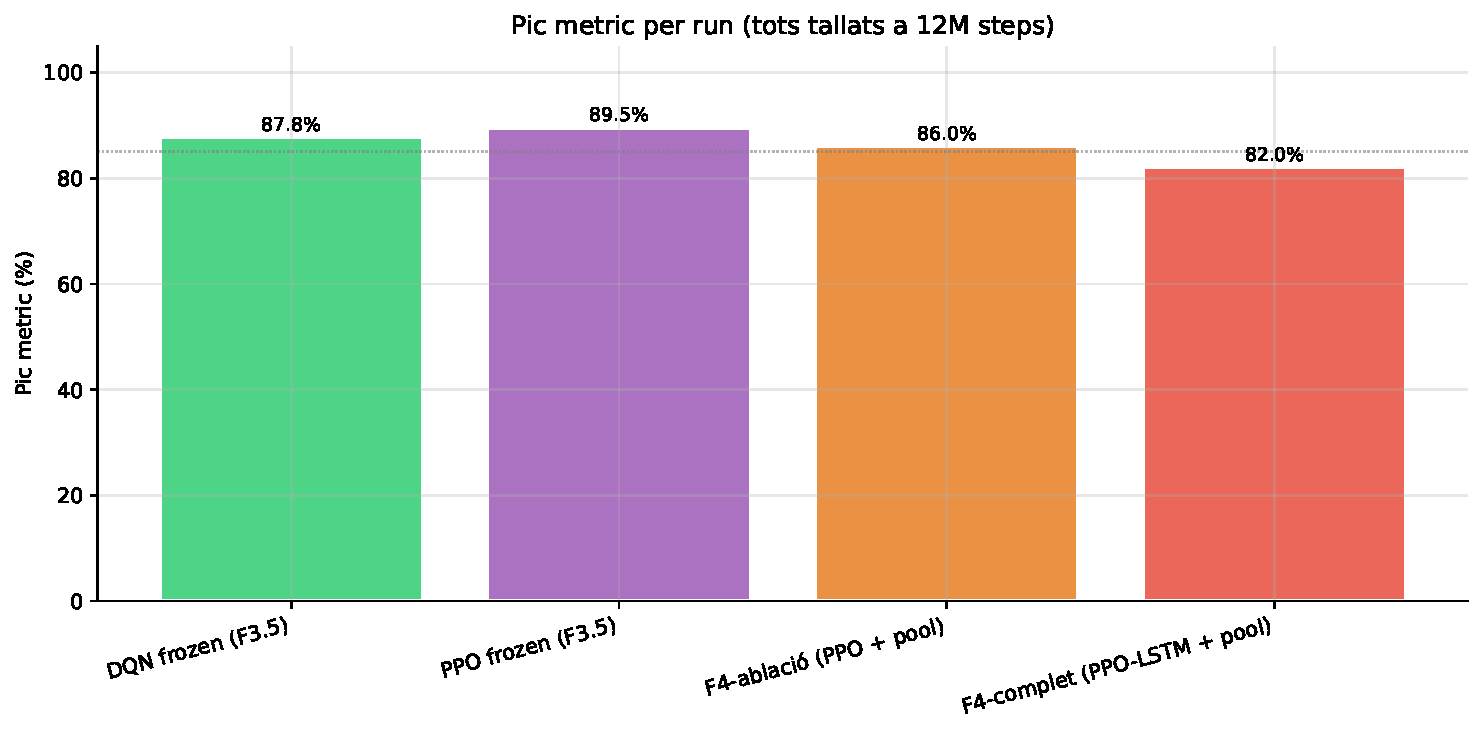
\includegraphics[width=\textwidth]{figures/fase4/fase4_barplot.pdf}
  \caption{Pic de \texttt{metric} per a cada run, tots tallats al pressupost comú de 12M
           passos. DQN~frozen assoleix 87{,}8\% dins el pressupost; el seu pic global és
           91{,}2\% a 23M passos.}
  \label{fig:fase4-barplot}
\end{figure}

\begin{figure}[H]
  \centering
  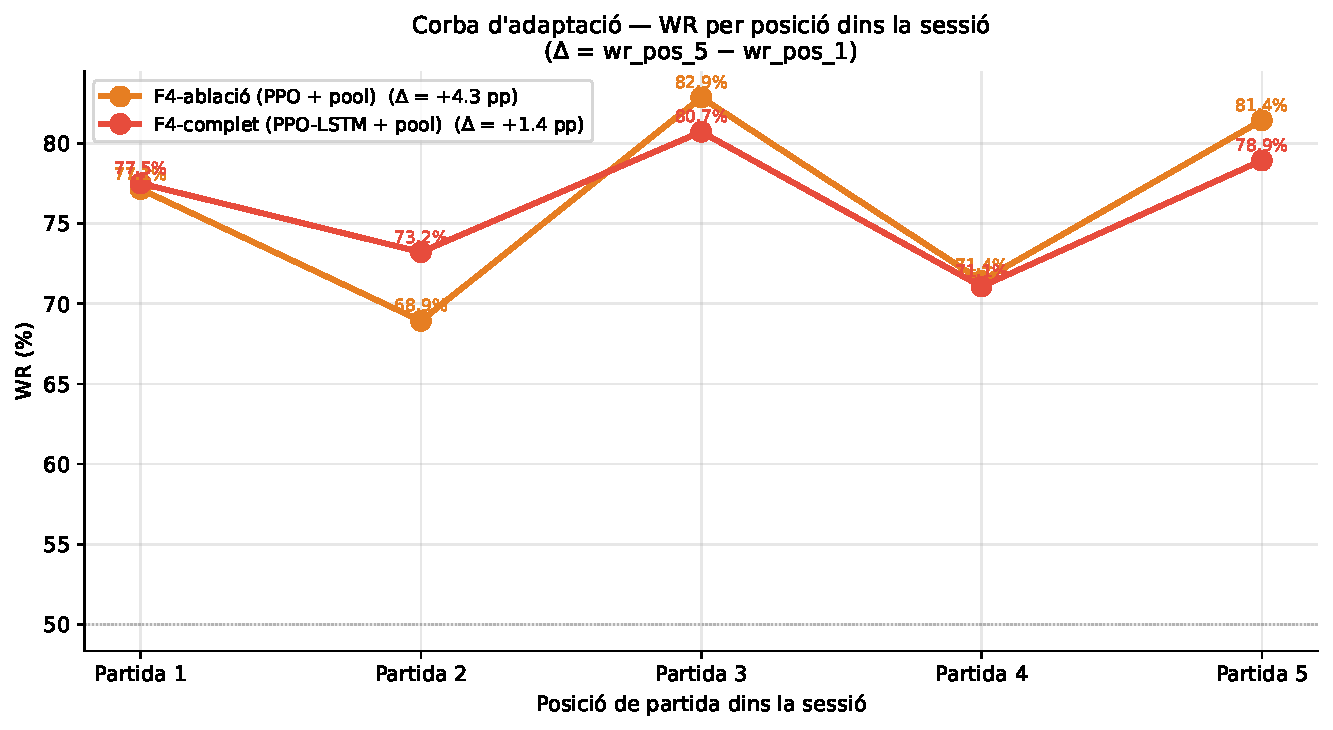
\includegraphics[width=\textwidth]{figures/fase4/fase4_adaptacio.pdf}
  \caption{Win-rate per posició dins la sessió (mà~1 a mà~5) per als dos runs de la
           Fase~4 (mitjana de les cinc darreres avaluacions). El $\Delta$ indica la
           diferència entre la mà~5 i la mà~1. La línia puntejada marca el 50\%.}
  \label{fig:fase4-adaptacio}
\end{figure}

\begin{table}[H]
  \centering
  \begin{tabular}{llrr}
    \toprule
    Run & Memòria & Pic \texttt{metric} (12M) & Temps \\
    \midrule
    DQN frozen (F3.5) & No            & 87{,}8\% & — \\
    PPO frozen (F3.5) & No            & 89{,}5\% & 0{,}33~h \\
    F4-ablació        & No            & 86{,}0\% & 0{,}33~h \\
    F4-complet        & \ac{LSTM} 256 & 82{,}0\% & 15{,}2~h \\
    \bottomrule
  \end{tabular}
  \caption{Resultats de la Fase~4 (pressupost igualat a 12M passos). DQN frozen mostra el
           seu màxim dins el pressupost de 12M; el seu pic global és del 91{,}2\% a 23M.}
  \label{tab:fase4}
\end{table}

\emph{H1: l'\ac{LSTM} millora el rendiment global.} \textbf{No es valida.}
F4-complet assoleix un 82{,}0\% de \texttt{metric}, \emph{4~punts per sota} de F4-ablació
(86{,}0\%), que entrena amb el mateix pool però sense memòria. A igual pressupost (12M
passos), la memòria no aporta cap guany global i a més eleva el cost computacional 46$\times$
(15{,}2~h vs 0{,}33~h).

\emph{H2: adaptació progressiva dins la sessió.} \textbf{No es valida.}
La corba de win-rate per posició (mà~1 a mà~5, figura~\ref{fig:fase4-adaptacio}) és
sorollosa i no monòtona: $[77{,}5;\,73{,}2;\,80{,}7;\,71{,}1;\,78{,}9]$,
$\Delta = +1{,}4$~punts. El patró no és gaire diferent del de F4-ablació (sense memòria),
la qual cosa descarta l'aprenentatge adaptatiu i apunta a un artefacte de la mida de
mostra (${\sim}56$~sessions per posició), insuficient per detectar tendències fiables.

\emph{H3: el pool no perjudica significativament la convergència.} \textbf{Parcialment
valida.} F4-ablació (86{,}0\%) queda 3{,}5~punts sota PPO frozen (89{,}5\%), just al
límit del criteri $\pm3$~punts. El pool dificulta lleugerament la convergència sense
memòria, però el delta és prou petit per no descartar la configuració.

La causa subjacent del fracàs de H1 i H2 és el \textbf{desajust entre entrenament i
avaluació}: s'entrena sobre sessions de 5~mans (${\sim}50$~passos), però s'avalua sobre
sessions de 5~partides senceres (${\sim}500$~passos), un context deu vegades més llarg que
la xarxa no ha vist mai. S'hi sumen el pressupost reduït (12M vs 24M de les línies base)
i les sessions d'entrenament massa curtes perquè la retropropagació en el temps propagui
senyals d'adaptació significatius.

\paragraph{Decisió.} Els resultats revelen marges de millora concrets. El canvi més crític
seria \textbf{alinear el context d'entrenament i d'avaluació}: substituir les sessions de
5~mans (${\sim}50$~passos) per sessions de partides senceres (${\sim}500$~passos), de
manera que la xarxa hagi vist durant l'entrenament el mateix horitzó temporal que a
l'avaluació. Un \textbf{\ac{LSTM} més petit} (64--128 unitats en lloc de 256) reduiria
el cost computacional i facilitaria la convergència; augmentar el \textbf{pressupost} fins
als 24M passos de les línies base i allargar les \textbf{seqüències de BPTT} donarien a
la memòria el temps i el context necessaris per propagar senyals d'adaptació reals.

Malgrat aquestes millores possibles, aquest \ac{TFG} descarta la línia de recerca
recurrent: amb H1 i H2 invalidades, H3 just al límit i un cost computacional 46$\times$
superior, la relació cost-benefici no justifica continuar-la dins del pressupost disponible.
La tria entre els candidats restants (F4-ablació i les línies base de la Fase~3.5) es
resol al Checkpoint~2.

\subsection{Checkpoint 2: model seleccionat}
\label{sec:checkpoint2}

Tancades les Fases~3 i~4, el model que s'adopta per a desplegament és \textbf{F4-ablació}
(PPO + COS congelat + pool, 86{,}0\% a 12M passos). La decisió pondera rendiment, robustesa
i cost.

La raó principal és la \textbf{robustesa davant estils diversos}. F4-ablació s'ha entrenat
contra les sis variants d'\texttt{AgentRegles}, de manera que la seva política és
generalista; les millors línies base de la Fase~3.5 (DQN i PPO frozen) van entrenar sempre
contra un oponent fix i no s'han enfrontat a aquesta diversitat. En un context de
desplegament real, on l'oponent és desconegut, aquesta generalitat és més valuosa que uns
quants punts de win-rate aconseguits contra un únic adversari. A això s'hi suma la
\textbf{rapidesa d'entrenament} (0{,}33~h per execució, davant les 15{,}2~h de F4-complet o
les diverses hores del DQN), que permet iterar i reentrenar amb facilitat, i un
\textbf{rendiment competitiu} al pressupost igualat (només 3{,}5~punts sota PPO frozen).

\textbf{DQN frozen} té el millor win-rate brut (91{,}2\% al pic global), però va ser entrenat
contra un oponent fix i no s'ha provat contra el pool; per això no es tria. . Finalment, l'\ac{LSTM} (F4-complet) queda
descartada: un cost 46$\times$ superior i un rendiment 4~punts inferior no compensen, i cap
de les seves hipòtesis s'ha validat.

Aquesta robustesa, però, encara no s'ha \emph{quantificat}: la \texttt{metric} clàssica
promitja entre oponents i pot amagar debilitats davant estils concrets. Mesurar-la i
millorar-la és l'objectiu del Bloc~3.
